\section{Анализ литературных источников, прототипов и формирование требований к проектируемому программному средству}
\label{sec:analysis}

Конечный успех программного проекта во многом определяется до начала конструирования: на этапе подготовки, которая проводится с учетом всех
особенностей проекта.

Первое предварительное условие, которое нужно выполнить перед конструированием, – ясное формулирование проблемы, которую система должна
решать. Общая цель подготовки — снижение риска: адекватное планирование
позволяет исключить главные аспекты риска на самых ранних стадиях работы,
чтобы основную часть проекта можно было выполнить максимально эффективно.

Главный факторы риска в создании ПО — неудачная выработка требований. Требования подробно описывают, что должна делать программная система. Внимание к требованиям помогает свести к минимуму изменения системы
после начала разработки \cite{book_makkonel}.

Перед формулированием требований необходимо изучить ряд вопросов,
которые напрямую влияют на все дальнейшие этапы разработки. В частности,
необходимо рассмотреть вопросы выбора платформ, архитектуры. По результатам анализа можно будет составить техническое задание к проектируемому программному средству, которое станет основой для составления функциональных требований.

\subsection{Аналитический обзор литературных источников}
\label{sec:analysis:literature}

Далее приводится анализ сведений, которые влияют на формулирование
требований, выбор архитектуры и дальнейшее проектирование и разработку
программного средства.

\subsubsection{} Кроссплатформенность программного обеспечения
\label{sec:analysis:literature:crossplatform}

В настоящее время выбор платформы является серьезным фактором во время всех этапов разработки, от правильно выбранной платформы зависит набор
возможных технологий, которые можно использовать при разработке программного продукта. Уже сейчас с каждым днем появляются все новые технологии,
которые позволяют переиспользовать однажны написанный код на других платформах \cite{habr_crossplatform}. Примером таких технологий являются C\# и Java. В их основе лежит
так называемый IL -- intermidiate language, своеобразный промежуточный язык, в который компилируется исходный код программы \cite{clr_csharp}. В дальнейшем на целевую платформу
устанавливается CLR - common language runtime или общая среда выполнения, которая читает код на промежуточном языке и представляет его в виде, понятном для 
целевой платформы \cite{clr_csharp}. Таким образом кроссплатформенность - это один из факторов, который необходимо учитывать при выборе техногии для реализации проекта.

\subsubsection{} Обзор целевых платформ
\label{sec:analysis:literature:target_platforms}

Несмотря на планируемое использование кроссплатформенных технологий, поддержка всех платформ может затребовать значительно больших средств и времени, чем есть в наличии 
для выполнения дипломного проектирования. Поэтому, необходимо осуществить выбор одной основной платформы с
расчетом на продолжение разработки и реализацию проекта для других платформ. Рассмотрим достоинства и недостатки основных.

\emph{Настольное приложение} – программное средство, которое запускается локально на компьютере пользователя. 
При его создании появляется возможность использования всех преимуществ аппаратного обеспечения, которым оснащен компьютер, например: прямой доступ к видеокарте, к устройствам
периферии. Кроме того, появляется возможность взаимодействия с другими установленными приложениями, а также в подавляющем числе случаев возможность автономной работы.
Тем не менее у настольных приложений есть и ряд недостатков. Когда
пользователь работает удаленно, возникают проблемы, связанные с сетью, соединениями, сетевыми экранами. Один из самых больших недостатков заключается в огромной сложности 
развертывания приложения на десятки или сотни
машин, их конфигурирования, периодического обновления \cite{msdn_desktop_vs_web}.

\emph{Веб-приложения}, в отличие от настольных, работают на удаленном аппаратном обеспечении и поставляются пользователю через браузер \cite{web_based_vs_desktop}. При
их использовании разработчик избавляется от необходимости поддерживать
установку большого числа зависимостей, он всегда может быть уверен, что
все пользователи используют самую последнюю версию приложения. Вычислительные операции могут производиться на мощном сервере, а результаты
вычислений поставляться пользователю – так называемая концепция «тонкого
клиента» \cite{desktop_vs_web_deeper_look}.

Несмотря на то, что ресурсоемкие вычисления производятся на сервере,
задержки при передаче, особенно при нестабильном соединении, сама потребность в постоянном интернет соединении могут значительно снизить удобство
пользования приложением. Кроме того, размер загружаемого при каждом запуске кода и ресурсов может значительно увеличить траты пользователя, особенно если он использует 
дорогое мобильное подключение к интернету.

Для \emph{мобильных приложений} актуальны ограничения платформ, на которых они запускаются, такие как меньшие размеры экранов, более медленные процессоры, 
ограниченное энергопотребление. Несмотря на это, мобильные устройства часто находятся рядом с пользователями, появляется возможность использования 
мгновенных оповещений \cite{desktop_mobile_differences}. Вместе с этим, большинство смартфонов оснащено модулями, такими как GPS, камера, NFC, 
что предоставляет разработчику новые возможности по их использованию.
На основании рассмотренных характеристик различных платформ можно
осуществить выбор одной из них, которая и станет целевой для разработки.

\subsubsection{} Обзор архитектурных стилей
\label{sec:analysis:literature:architecture_styles}

Далее необходимо рассмотреть применяющиеся на практике архитектурные стили, провести их анализ и по результатам осуществить выбор архитектуры, которая затем будет 
применяться при проектировании программного средства.

Под разработкой \emph{архитектуры} понимают специфицирование структуры
всей системы: глобальную организацию и структуру управления, протоколы
коммуникации, синхронизации и доступа к данным, распределение функциональности между компонентами системы, физическое размещение, состав системы, масштабируемость и 
производительность \cite{introduction_to_architecture}. Набор принципов, используемых в архитектуре, формирует \emph{архитектурный стиль}. Применение архитектурных 
стилей упрощают решение целого класса абстрактных проблем \cite{introduction_to_architecture}.

При проектировании архитектуры программной системы почти никогда
не ограничиваются единственным архитектурным стилем, поскольку они могут
предлагать решение каких-либо проблем в различных областях. В таблице ~\ref{table:analysis:literature:architecture_styles}
приведен вариант категоризации архитектурных стилей \cite{application_architecture_guide}.

\begin{table}[!h]
\caption{Категоризация архитектурных стилей}
\label{table:analysis:literature:architecture_styles}
\centering
    \begin{tabular}{{ 
    |>{\raggedright}m{0.35\textwidth} | 
        >{\raggedright\arraybackslash}m{0.60\textwidth}|}}

        \hline
    Категория & Архитектурный стиль \\
    
    \hline
    Связь & SOA (Service-oriented architecture – архитектура, ориентированная на сервисы), Шина сообщений \\

    \hline
    Развертывание & Клиент-серверный, трехуровневый, N-уровневый \\

    \hline
    Предметная область & DDD (Domain-driven design – проблемно-ориентированное проектирование) \\

    \hline
    Структура & Компонентный, объектно-ориентированный, многоуровневый\\

    \hline
    \end{tabular}
\end{table}

\emph{Сервис-ориентированная архитектура} позволяет приложениям пре-доставлять некоторую функциональность с 
помощью набора слабосвязанных автономных сервисов; связь между сервисами обеспечивается с помощью заранее определенных контрактов.
Данный стиль предоставляет следующие преимущества \cite{application_architecture_guide}:

\begin{itemize}
	\item повторное использование сервисов снижает стоимость разработки;
	\item автономность и использование формальных контрактов способст-вует слабой связанности и повышает уровень абстракции;
	\item сервисы могут использовать возможность автоматического обнаружения и определения интерфейса;
	\item сервисы и использующие их приложения могут быть развернуты на различных платформах.
\end{itemize} 

Архитектура \emph{шины сообщений} описывает принципы построения систем,
которые используют обмен сообщениями как способ связи. Наиболее часто при
реализации данной архитектуры используется модель маршрутизатора сообще
ний или шаблон издатель-подписчик. Главные преимущества использования
данного архитектурного стиля \cite{application_architecture_guide}:

\begin{itemize}
	\item расширяемость, которая заключается в возможности добавлять и удалять приложения без влияния на другие;
	\item снижается сложность приложений, так как единственный интерфейс, который они должны поддерживать – интерфейс общей шины;
	\item гибкость, которая заключается в возможности подстраиваться под бизнес-требования или желания пользователей через изменения конфигурации или параметров маршрутизации сообщений;
	\item слабая связанность, поскольку единственное, чем связаны приложения -- интерфейс общей шины;
  	\item масштабируемость, которая заключается в возможности в случае необходимости присоединения к шине нескольких экземпляров одного и того же приложения.
\end{itemize} 

\emph{Клиент-серверная архитектура} описывает распределенную систему, которая включает независимые системы сервера, клиента и соединяющую их
сеть. Иногда данную архитектуру называют двухзвенной. Из преимуществ выделяют следующие  \cite{introduction_to_architecture}:

\begin{itemize}
	\item безопасность: все данные хранятся на сервере, обеспечивающем больший уровень безопасности, чем отдельные клиенты;
	\item централизованный доступ к данным, который предоставляет возможность более легкого управления, чем в других архитектурах;
	\item устойчивость и легкость поддержки: роль сервера могут выполнять несколько физических компьютеров, объединённых в сеть; благодаря этому клиент не замечает сбоев или замены отдельного серверного компьютера.  
\end{itemize} 

\emph{Многоуровневый архитектурный стиль} заключается в группировании
схожей функциональности приложения по уровням, которые выстроены в вертикальную структуру. Уровни связаны слабо, связь между ними осуществляется по явно 
установленным протоколам. Строгий вариант архитектуры предполагает, что компоненты какого-либо уровня могут взаимодействовать только с
компонентами одного нижележащего уровня; ослабленный вариант разрешает
взаимодействие с компонентами любого из нижележащих уровней. Использование данного архитектурного стиля предлагает следующие преимущества
\cite{application_architecture_guide}:

\begin{itemize}
	\item есть возможность осуществлять изменения на уровне абстракций;
	\item изолированность: изменения на каких-либо уровнях не влияют на другие, что снижает риск и минимизирует воздействие на всю систему;
	\item разделение функциональности помогает управлять зависимостями, что приводит к большей управляемости всего кода;
  	\item независимые уровни предоставляют возможность повторного использования компонентов;
  	\item строго-определенные интерфейсы способствуют повышению тес-тируемости компонентов.
\end{itemize} 

\emph{Многозвенная архитектура} предлагает схожее с многоуровневой архитектурой разбиение функциональности, отличие же заключается в предлагаемом размещении 
звеньев на физически обособленной машине \cite{application_architecture_guide}. Предлагается использовать данный стиль в случаях, когда компоненты одного звена
могут проводить дорогие в ресурсном отношении вычисления, так что это может сказаться на других уровнях, или когда некоторую чувствительную информацию переносят 
со звеньев уровня представления на уровень бизнес-логики приложения. Далее приведены главные преимущества использования многозвенной архитектуры:

\begin{itemize}
	\item удобство сопровождения, которое заключается в возможности внесения изменений и обновлений в некоторые компоненты при минимальном влиянии на всё приложение;
	\item масштабируемость, которая возникает из распределенного развертывания;
	\item гибкость, которая появляется благодаря предыдущим двум пунктам;
  	\item масштабируемость также приводит к повышению доступности приложения.
\end{itemize} 

\emph{Проблемно-ориентированный архитектурный стиль} основывается на
предметной области, ее элементах, их поведении и связях между ними. Для
применениях данного стиля необходимо иметь хорошее понимание предметной области или людей, которые бы смогли объяснить ее специфику разработчикам. 
Первое, что нужно сделать при принятии данного стиля – выработать
единый язык, который бы знала вся команда разработчиков, который бы был
избавлен от технических жаргонизмов и содержал только термины предметной
области – только так можно избежать проблемы непонимания между участникам \cite{ddd_quickly}. Преимущества, которые может предложить данный стиль:

\begin{itemize}
	\item упрощение коммуникации между участниками процесса разработки благодаря выработке единого языка;
	\item модель предметной области обычно является расширяемой и гибкой при изменениях условий и бизнес-требований;
	\item хорошая тестируемость.
\end{itemize} 

\emph{Компонентная архитектура} основывается на декомпозиции системы в
отдельные функциональные или логические компоненты, которые раскрывают
другим компонентам только заранее определенные интерфейсы \cite{application_architecture_guide}. Преимущества данного подхода:

\begin{itemize}
	\item легкость развертывания, которая заключается в обновлении компонентов без влияния на другие;
	\item использование компонентов сторонних разработчиков позволяет \linebreak снизить расходы на разработку и поддержку;
	\item поддержка компонентами заранее определенных интерфейсов позволяет упростить разработку;
	\item возможность переиспользования компонентов также оказывает влияние на снижение стоимости.
\end{itemize} 

\emph{Объектно-ориентированный архитектурный стиль} выражается в \linebreak разделении функциональности системы на множество автономных объектов, 
каждый из которых содержит некоторые данные и набор методов поведения, свойственных объекту. 
Обычной практикой является определение классов, соответствующих объектам предметной области. 
Применение данного стиля предоставляет следующие преимущества \cite{application_architecture_guide}:

\begin{itemize}
	\item соотнесение классов программы и объектов реального мира делает программное средство более понятным;
	\item полиморфизм и принцип абстракции предоставляет возможность повторного их использования;
	\item инкапсуляция повышает тестируемость объектов;
	\item улучшение расширяемости, которое возникает благодаря тому, что изменения в представлении данных не оказывают влияния на внешний интерфейс объекта, что не ограничивает его способность взаимодействовать с другими объектами;
  \item высокая сцепленность объектов, которая достигается использованием разных объектов для разного набора действий.
\end{itemize} 

Таким образом, применение рассмотренных архитектур на этапе проектирования окажет большое влияние на успешность всего процесса разработки;
какие бы стили не были применены, можно быть уверенным в правильности
выбора за счет того, что у всех из них есть определенные и зачастую разные
преимущества.

\subsection{Обзор существующих аналогов}
\label{sec:analysis:analogues}

Для решения задач управления процессом проведения викторин и их создания могут использоваться различные средства. Рассмотрим каждую из задач в отдельности.

\subsubsection{} Управление процессом создания викторин
\label{sec:analysis:analogues:create_quest}

Для организаторов проведения викторин важнейшим аспектом является необмходимость в предварительно составленных викторинах по желаемой тематике.
Человеку известно тысячи различным областей знаний по самым разным предметам изучения и необходимо иметь возможность создать викторину по любой тематике, которая только может
придти в голову, причем для повышения уровня вовлеченности в игровой процесс следует использовать нечто большее, чем просто текст.

Одним из безусловных лидеров в области проведения викторин является программное средство SIGame, разработанное Владимиром Хилем. Для проведения викторин их необходимо предварительно 
создать в программном средстве, поставляемым отдельно под названием SIQuester. Данное программное средство позволяет создавать пакеты вопросов для дальнейшего использования
в SIGame. Интерфейс приложения выглядит как изображено на рисунке \ref*{sec:analysis:analogues:create_quest:siquester}.

\begin{figure}[!ht]
	\centering
	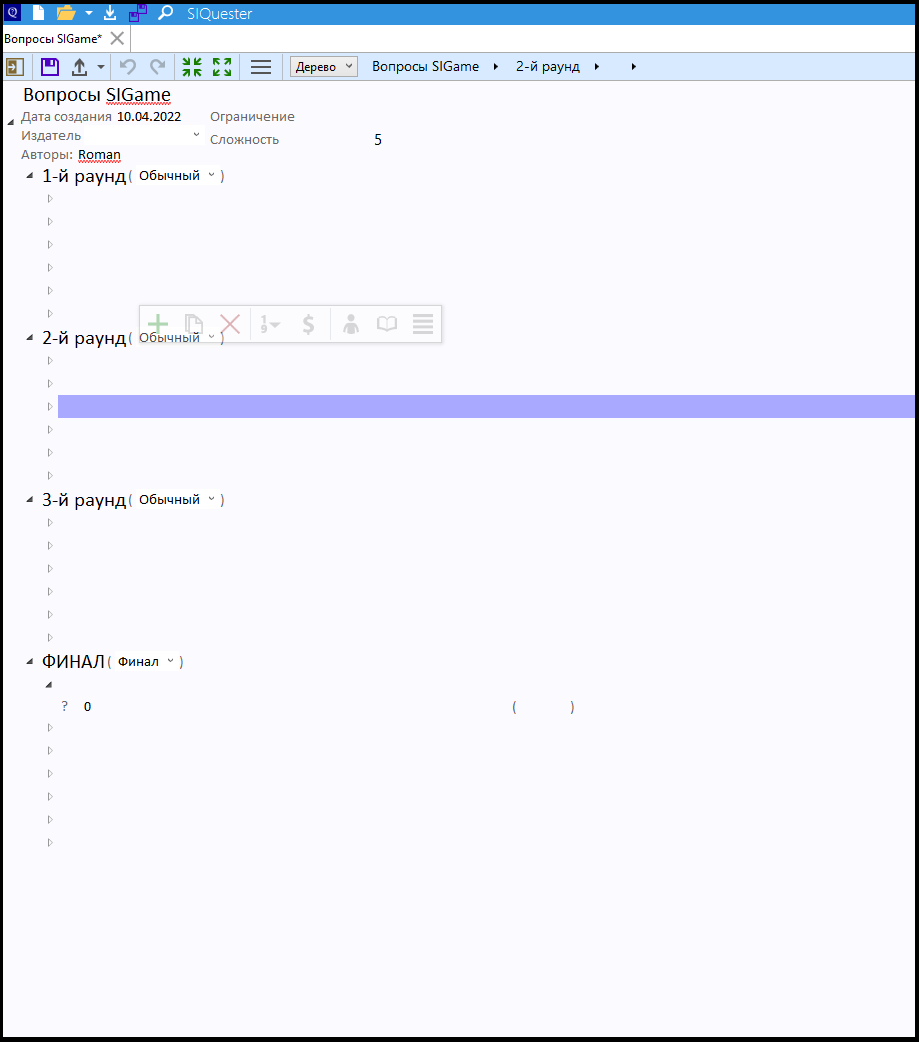
\includegraphics[scale=0.65]{attachments/siquester.png}  
	\caption{Интерфейс приложения SIQuester}
	\label{sec:analysis:analogues:create_quest:siquester}
\end{figure}

SIQuester поддерживает создание различных видов вопросов, как по содержанию, так и по формату разыгровки, среди поддерживаемых вопросов по содержанию есть:

\begin{itemize}
	\item текст;
	\item изображение;
	\item фрагмент видео;
	\item звуковой фрагмент.
\end{itemize} 

По формату разыгровки вопросов поддерживаются следующие варианты:

Простой вопрос -- отвечающий получает баллы в случае правильного ответа и теряет их в случае неверного ответа, это наболее частовстречающийся вопрос.

Вопрос со ставкой -- перед тем как игроки узнают содержимое вопроса происходит аукцион за право отвечать на вопрос. Тот, кто поставит больше очков и получить право отвечать на вопрос
при этом награда за правильный ответ или штраф за неправильный будет является финальным размером ставки на аукционе.

Вопрос с секретом -- тема вопроса, а также его стоимость может не совпадать с той, которая указана в сетке вопросов. В этом и заключается секретность вопроса. Этот вопрос также 
можно передать любому из участников.

Вопрос без риска -- в случае неправильного ответа участник, отвечающий на вопрос не теряет баллы, равные стоимости вопроса.

Примеры вопросов разных типов приведены на рисунке \ref*{sec:analysis:analogues:create_quest:siquester_types}.

\begin{figure}[!ht]
	\centering
	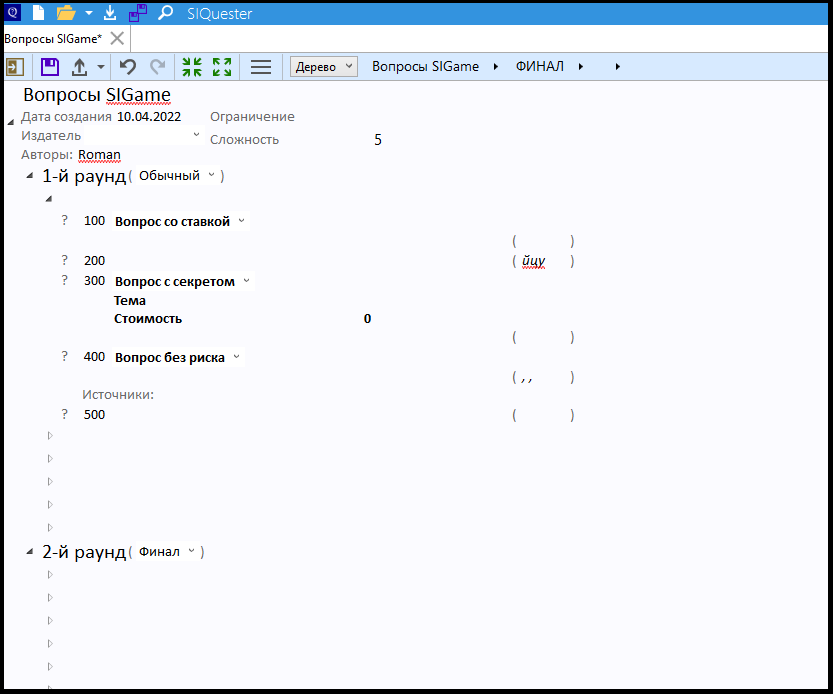
\includegraphics[scale=0.6]{attachments/siquester_types.png}  
	\caption{Примеры вопросов в SIQuester}
	\label{sec:analysis:analogues:create_quest:siquester_types}
\end{figure}

Анализ существующих аналогов по созданию вопросов показывает возможность наличия различных интерактивных видов вопросов для повышения заинтересованности игроков 
в игровом процессе и повышения уровня эмоционального удовлетворения в результате игры, но в то же время такой подход усложняет игровой процесс для совсем неопытных игроков,
поэтому в данном курсовом проекте будет использоваться единственный тип вопроса -- простой.

\subsubsection{} Управление процессом идентификации игроков
\label{sec:analysis:analogues:create_acc}

Для идентификации в сети в программном средстве используется анонимный подход: не нужны никакие средства внешней идентификации пользователя, такие как электронная почта,
номер телефона и так далее. Экран создания локального аккаунта для игры выглядит следующим образом (рисунок \ref{sec:analysis:analogues:create_acc:sigame_acc})

\begin{figure}[!ht]
	\centering
	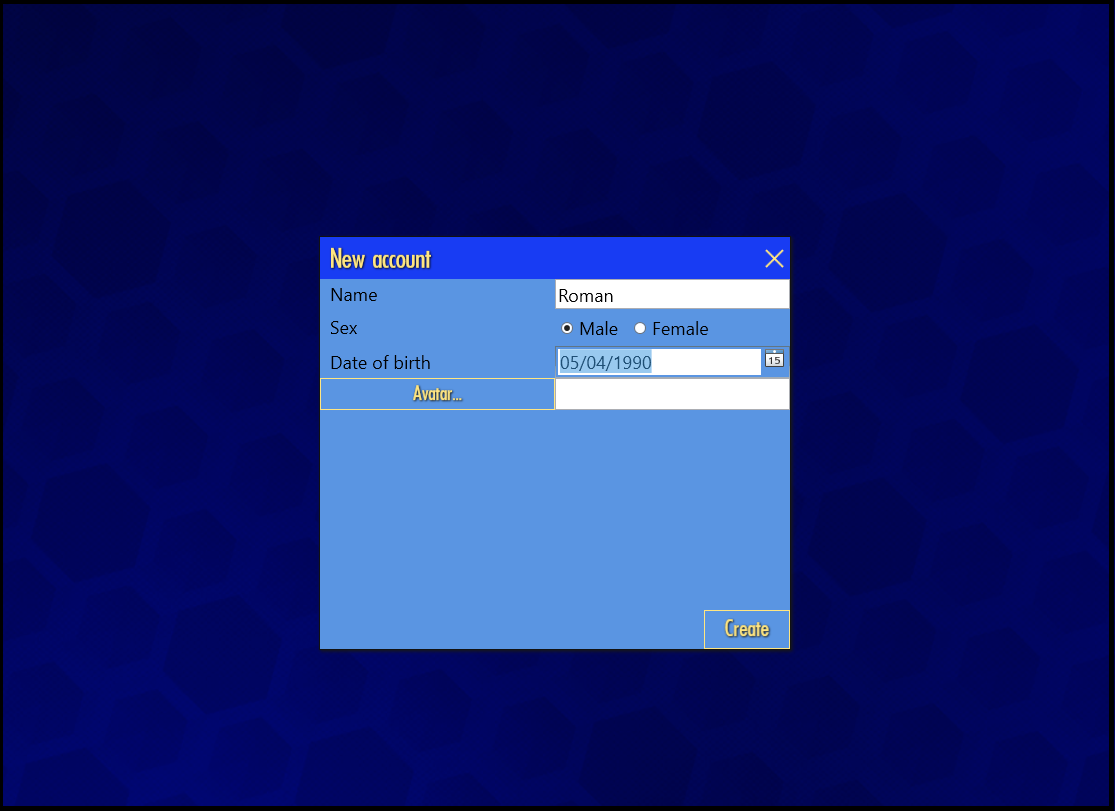
\includegraphics[scale=0.5]{attachments/sigame_acc.png}  
	\caption{Создание аккаунта в SIGame}
	\label{sec:analysis:analogues:create_acc:sigame_acc}
\end{figure}

Из этого можно сделать вывод, что аккаунты носят минимально функциональный характер и служит средством идентификации для
людей, которые и так уже знают игроков в реальной жизни, поэтому злоумышленник не сможет украсть какие-либо конфиденциальные данные,
так как приложение их нигде не хранит и не использует, а для проведения викторин они не требуются. 

Анализ показывает, что аккаунты в такого рода программных средствах используются лишь из необходимости минимальной идентификации в процессе игры и не служат для
сбора информации, поэтому смысла реализовывать какого либо рода защиту нет.

\subsubsection{} Управление процессом создания игры
\label{sec:analysis:analogues:host_game}

Перед тем как игроки смогут подключится к игре, необходимо, чтобы ведущий создал игровое лобби, пример реализации процесса создания лобби в SIGame изображен на 
рисунке \ref{sec:analysis:analogues:host_game:sigame_host}. 

\begin{figure}[!ht]
	\centering
	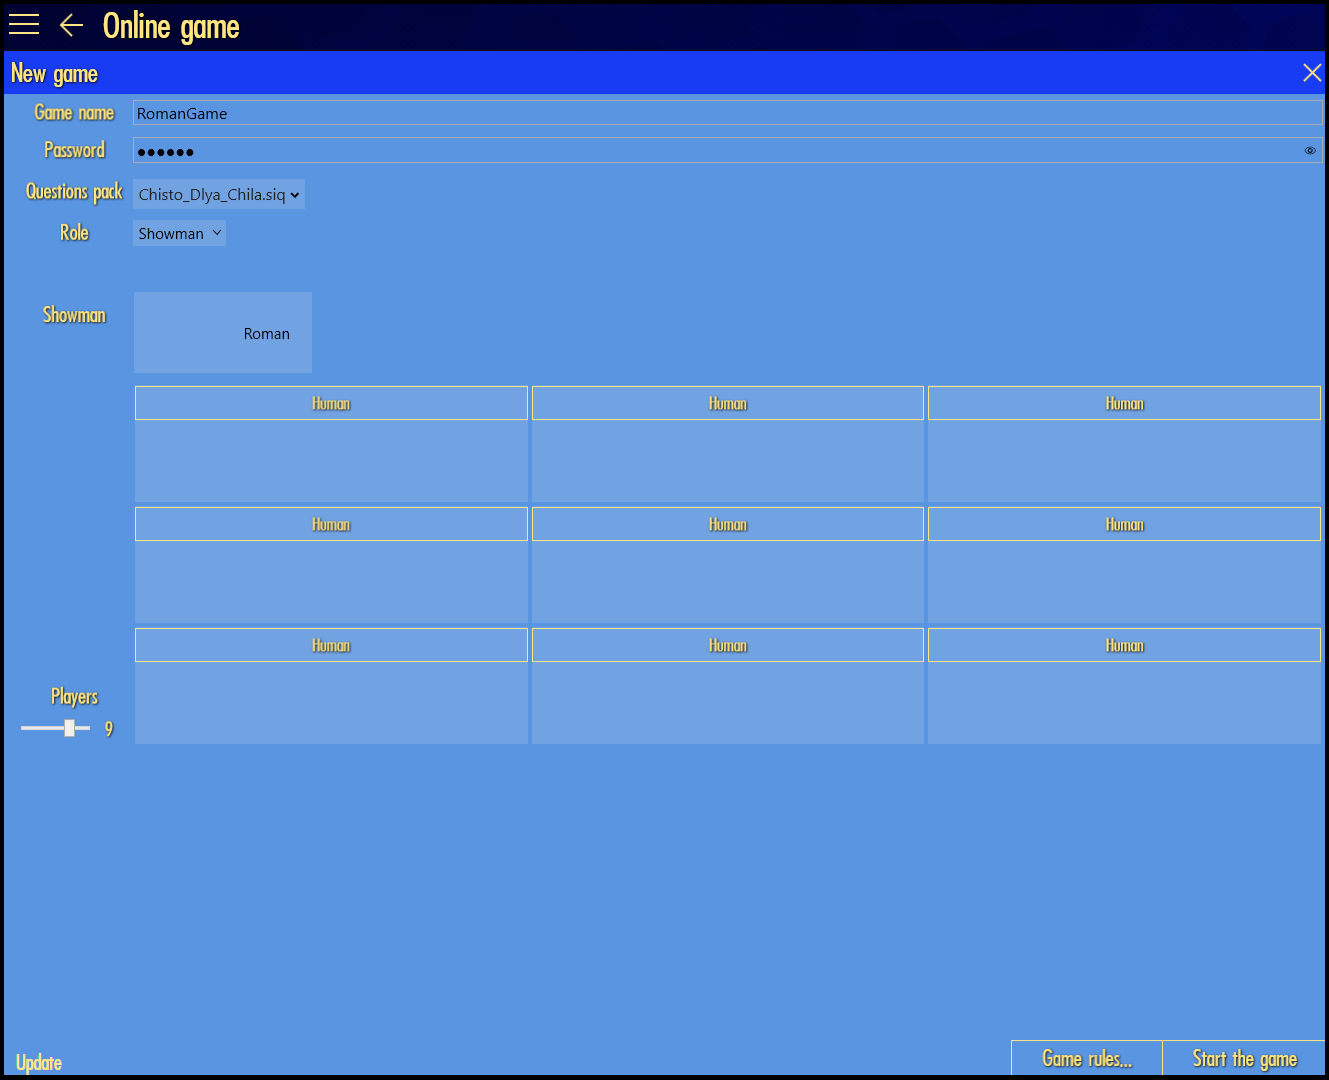
\includegraphics[scale=0.4]{attachments/sigame_host.png}  
	\caption{Создание игрового лобби в SIGame}
	\label{sec:analysis:analogues:host_game:sigame_host}
\end{figure}

Настройка лобби отвечает за несколько важных особенностей проведения викторины.

Название лобби позволяет игрокам, желающим присоединится к состязанию, найти игру в списке всех доступных игр, а зная название сделать это намного проще.

Пароль позволяет хосту защитить лобби от ограничить доступ нежелательным игрокам и оставить лишь тем, кто знает пароль.

Настройка вопросов позволяет выбрать заранее созданный в програм-ме тестере набор вопросов, на которые предстоит отвечать игрокам.

Размер игрового лобби позволяет устанавливать лимит на максимальное количество активных игроков в сессии, что позволит избежать слишком большого количества игроков в случае
создания игры без пароля.

Анализ показывает, что создание лобби это обязательная часть программного средства и от ее реализации зависит игровой опыт, который получат игроки в процессе проведения викторины.
Минимальный набор настроек, необходимых для настройки лобби были перечислены выше и требуются для дальнейшей реализации игрового процесса.

\subsubsection{} Управление процессом подключения к игре
\label{sec:analysis:analogues:join_game}

Игроки используют процесс подключения к игре, для того, чтобы попасть в одно игровое лобби с организатором викторины.
Процесс подключения к игровому лобби выглядит следующим образом (рисунок \ref{sec:analysis:analogues:join_game:sigame_join}).

\begin{figure}[!ht]
	\centering
	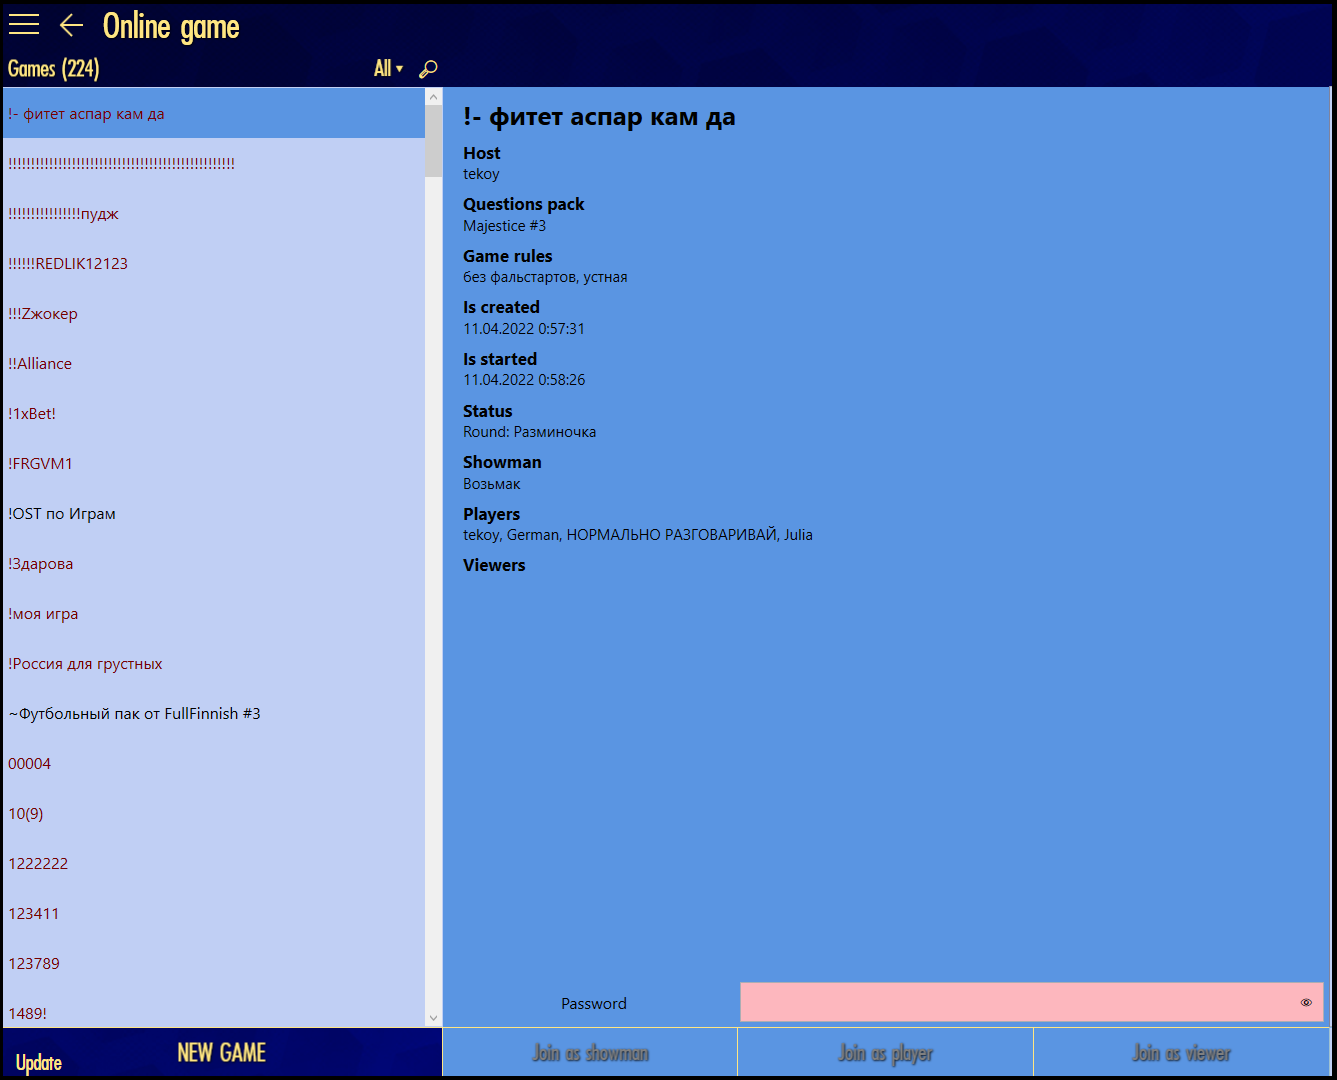
\includegraphics[scale=0.4]{attachments/sigame_join.png}  
	\caption{Подключение к игровому лобби в SIGame}
	\label{sec:analysis:analogues:join_game:sigame_join}
\end{figure}

Перед пользователем представлен список доступных игр для подключения, которые можно идентифицировать по названию игрового лобби и его организатору.
В случае, если лобби имеет пароль, то при подключении появляется модальное окно, где его необходимо ввести. После подключения пользователь попадает в лобби и 
может приступать к игровому процессу.

Анализ показывает, что процесс подключения к игре является одним из важнейших во всем программном средстве. Без возможности подключится к игровому лобби смысл
программного средства теряется.

\subsubsection{} Управление игровым процессом
\label{sec:analysis:analogues:game}

Игровой процесс заключается в поочередном ответе на вопросы и зачислении очков, победителем считается тот, кто набрал больше всего очков к моменту, когда закончатся все вопросы.
Фрагмент игрового процесса представлен на рисунке \ref{sec:analysis:analogues:game:sigame_game}.

\begin{figure}[!ht]
	\centering
	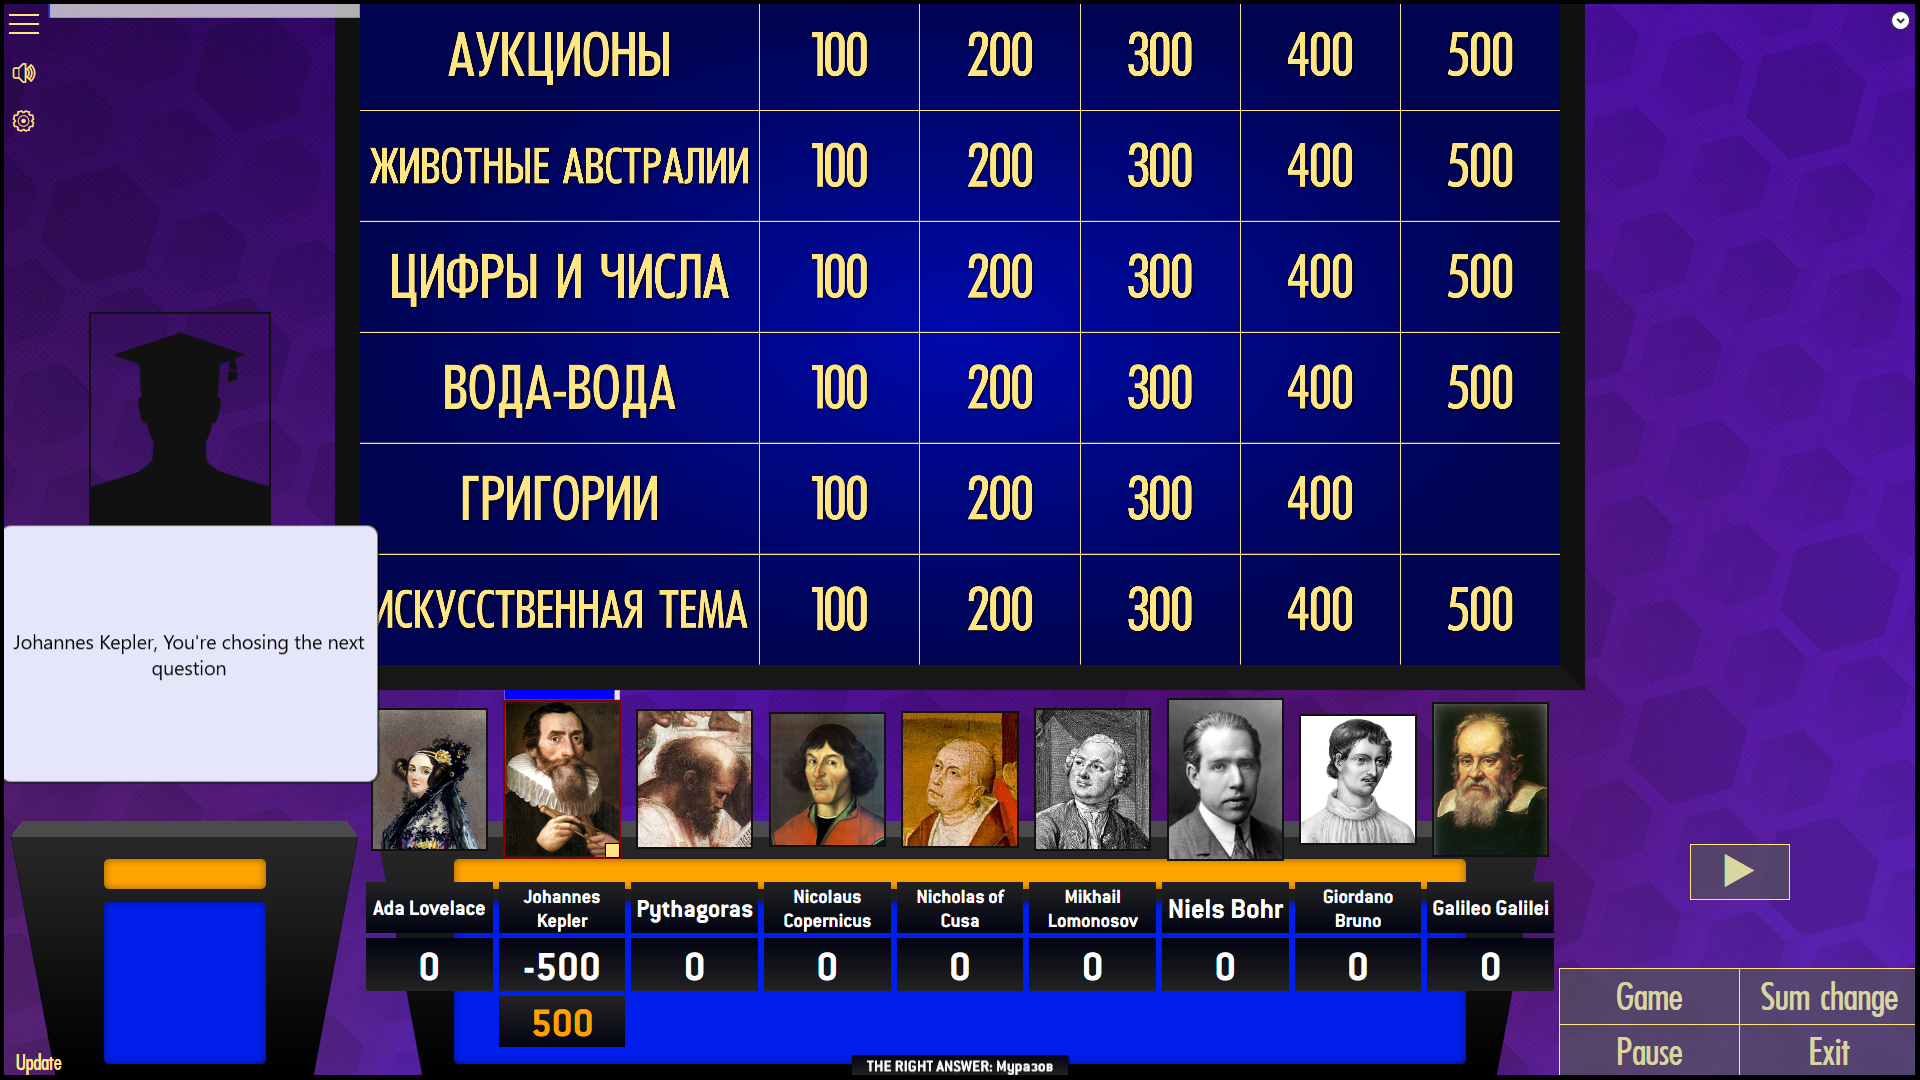
\includegraphics[scale=0.30]{attachments/sigame_game.png}  
	\caption{Процесс игры в SIGame}
	\label{sec:analysis:analogues:game:sigame_game}
\end{figure}

Следует отметить, что хотя сам игровой процесс является довольно простым, при этом он также является достаточно увлекательным, чтобы на долго время задерживать игроков и оставаться
увлеченным. Игроки отвечают на вопросы, в то время как ведущий контролирует правильность ответов и решает начислять очки, или нет. Здесь следует сделать оговорку, что предполагается,
что игра проходит в устной форме, т. е. игроки общаются между собой посредством внешнего программного средства для голосовой связи, например: Discord, Skype и так далее, поэтому реализация
средств коммуникации непосредственно в приложении не является необходимой.

Анализ показывает, что наибольшее внимание стоит уделить релизации логики игрового процесса, так как от него напрямую зависит удовлетворенность игроков процессом проведения викторин.

\subsubsection{} Обзор иных программных средств для проведения викторин
\label{sec:analysis:analogues:other_programs}

Рассмотренные процессы типичны для любого приложения с ориентацией на взаимодействие по сети, в то время как проведение викторин имеет свои особенности в разных реализациях.

Веб-аналоги позволяют избежать установки на персональный компьютер, но в то же время увеличивают нагрузку на сеть, что может быть не приемлемо для некоторых категорий пользователей.
К тому же в случае ограничения доступа к сайту или отказа в обслуживании больше воспользоваться программным средством не получится.

Реализации для мобильных телефонов имеют более скромный функционал по сравнению с версией для настольного компьютера, это обусловлено тем, что небольшой экран и нестабильное интернет-соединение
не могут обеспечить достаточный уровень комфорта при игре. К тому же общение с игроками затруднено тем, что использование средств связи на мобильном телефоне параллельно с проведением викторины
не является удобным, поэтому популярность такие реализации не снискали.

После анализа типичных реализаций был сделан вывод, что наилучшим решением для разработки программного средства проведения многопользовательских викторин является настольное приложение.


\subsection{Требования к проектируемому программному средству}
\label{sec:analysis:requirements}

По результатам изучения предметной области, анализа литературных источников и обзора существующих систем-аналогов сформулируем требования к проектируемому программному средству.

\subsubsection{} Назначение проекта
\label{sec:analysis:requirements:designation}

Назначением проекта является разработка программного средства, позволяющего автоматизировать процессы проведения викторин на произвольные темы.

\subsubsection{} Основные функции
\label{sec:analysis:requirements:functions}

Программное средство должно поддерживать следующие основные функции:

\begin{itemize}
	\item создание и редактирование пакетов с вопросами, которые будут использоваться во время проведения викторин;
	\item поддержка нескольких форматов вопросов (текст, звук, видео и т. д.);
	\item поддержка нескольких видов вопросов (обычный, с секретом, со ставкой и т. д.);
	\item анонимная авторизация с помощью локально созданного аккаунта;
	\item создание игрового лобби, как организатор викторины;
	\item настройка игрового лобби для проведения викторины (выбор пакета вопросов, пароль и т. д.);
	\item присоединение к игровому лобби в качестве игрока;
	\item управление игровым процессом для ведущего;
	\item автоматическое определение победителя после ответов на все вопросы.
\end{itemize} 

\subsubsection{} Требования к входным данным
\label{sec:analysis:requirements:input}

Входные данные для программного средства должны представлять из себя вводимый с клавиатуры текст или выбор доступных опций на пользовательском интерфейсе.
Должны быть реализованы проверки вводимых данных на корректность с отображением информации об ошибка в случае их некорректности.

\subsubsection{} Требования к выходным данным
\label{sec:analysis:requirements:output}

Выходные данные программного средства должны быть представлены посредством отображения информации с помощью различных элементов пользовательского интерфейса.

\subsubsection{} Требования к временным характеристикам
\label{sec:analysis:requirements:time}

Производительность программно-аппаратного комплекса должна \linebreak обеспечивать следующие временные характеристики: время реакции на запрос пользователя не должно
превышать одной секунды при минимальной скорости соединения 1 МБит/c. Допускается невыполнение данного требования в случае, когда невозможно обеспечить заявленную
пропускную способность интернет-канала по внешним причинам и не зависящим от пользователя обстоятельствам.

\subsubsection{} Требования к надежности
\label{sec:analysis:requirements:reliability}

Надежное функционирование программы должно быть обеспечено выполнением следующих организационно-технических мероприятий:

\begin{itemize}
	\item организация бесперебойного питания;
	\item выполнение требований ГОСТ 31078-2002 «Защита информации. Испытания программных средств на наличие компьютерных вирусов»;
	\item выполнение рекомендаций Министерства труда и социальной защиты РБ, изложенных в Постановлении от 23 марта 2011 г. «Об утверждении норм времени на работы по обслуживанию персональных электронно-вычислительных машин, организационной техники и офисного оборудования»;
	\item необходимым уровнем квалификации пользователей.
\end{itemize} 

Время восстановления после отказа, вызванного сбоем электропитания технических средств (иными внешними факторами), 
нефатальным сбоем операционной системы, не должно превышать времени, необходимого на перезагрузку операционной системы и запуск программы, 
при условии соблюдения условий эксплуатации технических и программных средств. Время восстановления после отказа, вызванного неисправностью технических средств,
фатальным сбоем операционной системы, не должно превышать времени, требуемого на устранение неисправностей технических средств и переустановки программных средств.

Отказы программы возможны вследствие некорректных действий \linebreak пользователя при взаимодействии с операционной системой. 
Во избежание возникновения отказов программы по указанной выше причине следует обеспечить работу конечного пользователя без предоставления ему административных привилегий.

\subsubsection{} Требования к аппаратному обеспечению серверной части
\label{sec:analysis:requirements:hardware_server}

ЭВМ, на которой должна функционировать серверная часть програм-много средства, должна обладать следующими минимальными характеристиками:

\begin{itemize}
	\item процессор Intel Core i7 с тактовой частотой 4 ГГц;
	\item жесткий диск объемом 100 Гб;
	\item оперативная память 16 Гб;
	\item сетевая карта Ethernet 100 МБит/с.
\end{itemize} 

Также для функционирования серверной части требуется Docker, который является кроссплатформенным программные средством, вследствие чего вопрос о целевой операционной системе не
рассматривается. Кроме того, процедуры установки и настройки данного программного средства выходят за рамки данного проекта и также не рассматриваются.

\subsubsection{}Требования к аппаратному обеспечению клиентской части
\label{sec:analysis:requirements:hardware_client}

Клиентская часть программного средства должна функционировать на ЭВМ со следующими минимальными характеристиками:
\begin{itemize}
	\item процессор Intel Core i7 с тактовой частотой 4 ГГц;
	\item оперативная память 4 Гб;
	\item сетевая карта Ethernet 10/100 МБит/с.
\end{itemize} 

Для корректной работы программного средства необходимы следующие программные компоненты:
\begin{itemize}
    \item операционная система Windows 10;
	\item .NET Framework 4.8;
	\item visual c++ redistributable.
\end{itemize} 

\subsubsection{}Выбор технологий программирования
\label{sec:analysis:requirements:language}

Язык программирования, на котором будет реализована система, имеет большое значение, так как он будет использоваться с начала конструирования программы и до самого конца.
Исследования показали, что выбор языка программирования несколькими способами влияет на производительность труда программистов и качество создаваемого ими кода. Если язык
хорошо знаком программистам, они работают более производительно. Данные, полученные при помощи модели оценки Cocomo II, показывают, что программисты, использующие язык, 
с которым они работали три года или более, примерно на 30\% более продуктивны, чем программисты, обладающие аналогичным опытом, но для которых язык является новым \cite{software_cost_estimation}.
В более раннем исследовании, проведенном в IBM, было обнаружено, что программисты, обладающие богатым опытом использования языка программирования, были более чем втрое 
производительнее программистов, имеющих минимальный опыт \cite{method_of_programming_measurement_and_estimation}.

Язык программирования С\#, указанный в задании на дипломное проектирование, является кроссплатформенным языком программирования и является частью платформы .NET. Данный ЯП представляет собой самостоятельный язык, 
который имеет C-образный синтаксис и семантику управляющих конструкций. Так как язык является строго типизированным, то основные ошибки можно отловить еще на этапе компиляции проекта.
Свою популярность он снискал за небольшое количество легаси-кода и большое количество синтаксического "сахара", который позволяет компактно описывать сложные конструкции.
Еще одной сильной стороной является технология LINQ, которая позволяет работать с любыми коллекциями, будь то база данных или локальный массив одинаково, причем в стандарте уже
реализованы все основные операции работы с данными, такие как добавление, обновление, удаление, фильтрация и так далее. Язык компилируется в IL и в дальнейшем выполняется в 
CLR, что обеспечивает кроссплатформенность и поддержку принципа write once -- run anywhere (напиши один раз -- запуская везде).
На данном языке разработано множество библиотек для работы в самых разных областях, например: настольные приложения, веб-приложения, машинное обучение и так далее. Таким
образом программист, знающий С\#, может писать под что угодно, лишь за исключением систем, для которых объем памяти строго ограничен, к таким относятся встраиваемые системы.

Среди достоинств платформы .NET можно выделить следующие:

\begin{itemize}
	\item обеспечение согласованной объектно-ориентированной среды программирования для локального сохранения и выполнения объектного кода, для
    локального выполнения кода, распределенного в Интернете, либо для удаленного выполнения;
	\item обеспечение среды выполнения кода, минимизирующей конфликты
    при развертывании программного обеспечения и управлении версиями;
	\item обеспечение среды выполнения кода, гарантирующей безопасное выполнение кода, включая код, созданный неизвестным или не полностью доверенным сторонним изготовителем;
	\item обеспечение среды выполнения кода, исключающей проблемы с производительностью сред выполнения сценариев или интерпретируемого кода;
	\item обеспечение единых принципов работы разработчиков для разных типов приложений, таких как приложения Windows и веб-приложения;
	\item разработка взаимодействия на основе промышленных стандартов, которое обеспечит интеграцию кода платформы .NET с любым другим
    кодом.
\end{itemize} 

Исходя из достоинств данного языка программирования, можно сделать вывод, что он наиболее подходящий для решения проблем,
схожих с поднимаемыми в данной пояснительной записке. Именно поэтому С\# и выбран как основной язык программирования в задании к текущему дипломному проекту.
Он является простым, современным, объектно-ориенти-рованным, обеспечивающим безопасность типов языком программирования. Он соответствует международному стандарту Европейской ассоциации производителей компьютеров — стандарт ECMA-334, а
также стандарту Международной организации по стандартизации (International
Standards Organization, ISO) и Международной электротехнической комиссии
— стандарт ISO/IEC 23270. Компилятор Microsoft С\# для .NET согласуется с обоими этими стандартами \cite{msdn_charp}.

Передовой средой программирования, которая поддерживает С\# явля-ется Microsoft Visual Studio, которая входит в линейку
продуктов компании Microsoft, включающих интегрированную среду разработки программного обеспечения и ряд других инструментальных средств. Она
включает в себя редактор исходного кода с поддержкой технологии IntelliSense
и возможностью рефакторинга кода. Встроенный отладчик может работать как
отладчик уровня исходного кода, так и как отладчик машинного уровня. Visual
Studio позволяет создавать и подключать сторонние дополнения для расширения функциональности практически на каждом уровне, включая добавление
поддержки систем контроля версий исходного кода, добавление новых наборов инструментов или инструментов для прочих аспектов процесса разработки
программного обеспечения. Именно поэтому она и выбрана в качестве основной среды программирования.

Для разработки сервиса-координатора, который будет работать на сервере будет также использоваться С\# и технология сокетов с написанием собственного протокола передачи данных.
Данный протокол является необходимым по той причине, что клиентам и серверу необходимо понимать формат пакетов, приходящих друг от друга. Разрабатываемый сервер представляет из себя
приложение-сервис, которое работает постоянно и отвечает на запросы клиентов, при этом оно хранит некое промежуточное состояние работы, которое может использовать
при обработке запросов от клиентов. В случае разработки проектируемого программного средства веб-сервис будет хранить список активных игровых лобби, которые будут запрашивать
клиенты при попытке подключится к организатору викторины, а также игровые состояния для каждого лобби.

Сформулированные требования позволят осуществить успешное проектирование и разработку программного средства.


